\documentclass[10pt,twocolumn]{article}
\usepackage[a4paper,margin=15mm]{geometry}
\usepackage{amsmath,amssymb}
\usepackage{amsthm}
\usepackage{graphicx}
\theoremstyle{plain}
\newtheorem{theorem}{Theorem}
\newtheorem{proposition}[theorem]{Proposition}
\newtheorem{corollary}[theorem]{Corollary}
\theoremstyle{definition}
\newtheorem{definition}[theorem]{Definition}
\theoremstyle{remark}
\newtheorem{remark}[theorem]{Remark}
\usepackage{booktabs,array,calc}
\usepackage[font=small,labelfont=bf]{caption}
\usepackage[colorlinks=true]{hyperref}
\usepackage{etoolbox}
\providecommand{\tightlist}{\setlength{\itemsep}{0pt}\setlength{\parskip}{0pt}}
\renewcommand{\thesubsection}{\arabic{subsection}.}
\emergencystretch=3em
\allowdisplaybreaks
\setlength{\tabcolsep}{3.6pt}
\AtBeginDocument{%
  \BeforeBeginEnvironment{equation}{\small}%
  \BeforeBeginEnvironment{equation*}{\small}%
  \BeforeBeginEnvironment{align}{\small}%
  \BeforeBeginEnvironment{align*}{\small}%
  \BeforeBeginEnvironment{gather}{\small}%
  \BeforeBeginEnvironment{gather*}{\small}%
}

\begin{document}
\title{Probabilistic Sufficiency for the Obstruction Calculus:\\
Belief-State Safety Values under Partial Observation}
\author{Amin Abaee\\[0.35em]
{\small Independent Researcher}\\[0.55em]
{\small\href{https://orcid.org/0000-0002-0019-1842}{ORCID: 0000-0002-0019-1842}}\\[0.3em]
{\small\href{mailto:amin\_abaee@ut.ac.ir}{amin\_abaee@ut.ac.ir}}}
\date{September 26, 2026}
\maketitle

\begin{abstract}
The obstruction calculus characterizes nonviability through certificates on
information states; the probabilistic side asks what the certificates imply
when the information state is a distribution. This paper develops the
belief-state safety value \(V_{k}(b)\) --- the maximal probability of
remaining safe for \(k\) steps --- as a theory carried entirely in exact
rational arithmetic, with five results. First, a support identity: on
finite models with deterministic kernels and deterministic observation
maps the posterior support coincides with the set-valued post-state of the
calculus, the value-one level of the recursion coincides with the
viable-set recursion \(\mathcal{W}_{k}\), and outside it the deficit
satisfies \(1 - V_{k}(b) \ge \min_{x \in \mathrm{supp}(b)} b(x)\), attained
on natural instances; moreover the alpha-vectors are exactly the
indicators of the maximal jointly survivable subsets of the support ---
an antichain, Sperner-bounded --- which explains why the audited witness
census realizes three types. Second, exactness and parametric closed
forms: over rational input data the finite-horizon values are piecewise
linear with rational alpha-vectors, and on the delayed hidden-regime
class both the declared hold-class and the open-loop values are proved in
closed form for all initial states, all window lengths and horizons, and
all prior weights --- value one exactly on
\(z_{0} \ge 1 + \min(k, T_{\mathrm{obs}})\) and on \(z_{0} \ge 2\)
respectively, the larger prior mass off those regions, zero below the
floor --- so the complete \(16 \times 12\) audited value table, the
36/156 census, and the 384 hold-direction witnesses (348 distinct after
deduplication) become one-line corollaries. Third, the class lattice:
declared hold \(\subseteq\) open-loop \(\subseteq\) sequential
\(\subseteq\) fully observed orders the values, and both gaps are
realized exactly --- the value of flexibility on the timing cells and the
value of observation on the common-action cells, each \(\tfrac{1}{2}\) at
the symmetric prior and zero elsewhere. Fourth, agreement and
stabilization: the segment-form enumeration reproduces the closed forms
on all 48 audited cells and horizons \(k \le 4\), the certificate
partition coincides with the value boundaries, the hold-class value jumps
by exactly \(\tfrac{1}{2}\) at \(z_{0} = 1 + \min(k, T_{\mathrm{obs}})\),
the two classes differ exactly where
\(2 \le z_{0} < 1 + \min(k, T_{\mathrm{obs}})\) (on the audited grid,
exactly the timing cells, 36 combinations), and the value is frozen once
\(k \ge T_{\mathrm{obs}}\) on the finite survivable-set lattice, so the
audited tables are complete. Fifth, a genuinely stochastic layer: an
exact weighted-path deficit identity under noisy observation --- the
deficit is the prior mass weighted by fatal-reading probabilities, and a
two-state sensor instance attains deficit \(1/20\) against a minimal mass
of \(1/2\), so the min-mass bound is not universal there --- a
noisy-probe deadline family with three-valued exact values, and the
repetition trade-off: a second probe cuts the misread probability from
\(1/10\) to \(7/250\), and each probe step costs \(1/10\) of floor
margin. Every closed form is verified against brute-force enumeration
from the definitions, including a seeded randomized battery.
\end{abstract}

\textbf{Keywords:} partially observable control; viability kernels;
belief states; safety values; exact arithmetic; adaptive observation

\subsection{Introduction}\label{introduction}

Viability under incomplete observation divides into a necessity side and a
sufficiency side. The obstruction calculus treats the necessity side:
certificates whose firing proves nonviability of an information state
(Abaee, 2026b). The probabilistic question is the quantitative counterpart.
If the controller holds a distribution \(b\) over states rather than a set,
how safe is safe? The answer is a function: the belief-state safety value
\(V_{k}(b)\), the maximal worst-case probability of keeping the state
trajectory in the safe set for \(k\) steps. Its value-one level is the
viability statement of the set-valued theory; everything below level one
is measured by the deficit \(1 - V_{k}(b)\), and the obstruction
certificates reappear as lower bounds on that deficit.

This paper develops the probabilistic layer of the viability theory of
Abaee (2026b): the calculus there is set-valued, and the present theory
quantifies what remains safe once the information state is a
distribution. It brings together the stochastic selector development, the
belief-state value campaign, and the hidden-parameter learning-deadline
audit into one theory with parametric closed forms, a class lattice, and
an exact stochastic layer; the companion papers (the calculus, its
computational certification, and the worked-systems audit) are unaffected,
and nothing verified in them is re-proved differently here.

The development proceeds in seven steps. Section \ref{model} states the
augmented model --- total transition rows, an absorbing unsafe state
carrying its own observation, masked witnesses --- and the value recursion,
distinguishing the selector's attaining set from its value-one level.
Section \ref{support} connects the belief-state recursion to the
set-valued recursion of the calculus exactly, through the support of the
belief. Section \ref{exact} shows the finite-horizon values are piecewise
linear and exactly representable, and carries the complete audited value
table over the delayed grid. Section \ref{deterministic} evaluates the
deterministic limit, at which the recursion degenerates to a
survived-mass formula over blind action sequences, with the asymmetric
audit carried sequence by sequence. Section \ref{deficit} reads the
obstruction certificates systematically as deficit lower bounds. Section \ref{agreement} proves agreement between the declared-class
segment enumeration and the closed-form values on the audited
delayed-regime class,
quantifies what the class declaration contributes, locates the value's
jump loci, and carries the derivations. Section \ref{adaptive} treats
observation as a design variable: probes, learning deadlines, and the
exact kernel cost of late resolution of a hidden parameter.

\emph{Relation to prior work.} The belief-support reduction at the core
of Theorem \ref{thm:support} is the finite-horizon qualitative analysis
of partially observable Markov decision processes: almost-sure safety
depends only on belief supports, as established for qualitative
objectives by Chatterjee, Doyen, and Henzinger (2009). What is added
here is quantitative and structural: the deficit bound and its witness
reading (Propositions \ref{prop:pl} and \ref{prop:deficit}), the
survivable-set (antichain) formula behind the witness census
(Proposition \ref{prop:antichain}), the class lattice with its realized
gaps (Theorem \ref{thm:lattice}), the parametric closed forms
(Proposition \ref{cor:closed} and Theorem \ref{thm:parametric}), and the
class-scoped timing obstruction. On complexity, finite-horizon partially
observable problems are PSPACE-complete and their no-observation variant
NP-complete (Papadimitriou and Tsitsiklis, 1987); the exponential
witness-growth law of Proposition \ref{prop:pl} is the honest general
behaviour, and the audited two-witness families are structural rather
than representative. Runtime safety filters for learning agents
(Alshiekh et al., 2018) and distributionally robust partially observable
models over ambiguity sets (Nakao, Jiang, and Shen, 2021), whose value
functions remain piecewise linear, bound the present development from
the computational and the modelling side; Section \ref{scope} records
the ambiguity-set interpolation as the formal home of worst-case
wording.

All audited computations are exact: integer and rational arithmetic,
standard library only, deterministic scripts (Section \ref{methods}).

\subsection{The augmented model, the safety value, and the selector}\label{model}

\emph{The augmented state space.} Let the physical safe set be
\(\mathcal{V}\) and let the state space of the model be
\(X^{\perp} = \mathcal{V} \cup \{\bot\}\), where \(\bot\) is an absorbing
unsafe state. For \(x \in \mathcal{V}\) the transition row splits between
\(\mathcal{V}\) and \(\bot\),
\[
\textstyle\sum_{x' \in \mathcal{V}} T(x' \mid x, a) \le 1,\quad
T(\bot \mid x, a) = 1 - \sum_{x' \in \mathcal{V}} T(x' \mid x, a),
\]
and the bottom row is \(T(\bot \mid \bot, a) = 1\): every row of \(T\)
sums to one and \(\bot\) is absorbing, so exit from \(\mathcal{V}\) is
absorption and no trajectory re-enters \(\mathcal{V}\) from outside it.
The observation model is completed on all of \(X^{\perp}\): there is a
distinguished observation \(y_{\bot}\) with
\(g(y_{\bot} \mid \bot, a, \bot) = 1\) (and
\(g(y \mid \cdot, \cdot, \bot) = 0\) for \(y \ne y_{\bot}\)), while
\(g(\cdot \mid x, a, x')\) on \(\mathcal{V}\) is arbitrary non-negative
with the usual normalization per \((x, a)\). A belief is a distribution
\(b\) over \(X^{\perp}\), updated by Bayes' rule \(\tau(b, a, y)\), with
\(\mathbb{P}(y \mid b, a) = \sum_{x, x'} b(x)\, T(x' \mid x, a)\,
g(y \mid x, a, x')\); because every row sums to one and every
\((x, a, x')\) emits exactly one observation with probability one, the
laws \(\mathbb{P}(y \mid b, a)\) sum to one over \(y\) at every belief ---
no sub-probability bookkeeping is needed. On the deterministic kernels of
the audited instances this formalism converts set-valued nonviability into
almost-sure nonviability on the augmented chain.

\begin{definition}[safety value]\label{def:value}
Fix a declared policy class \(\Pi\). The safety value at horizon \(k\) is
the maximal class-survival probability
\[
V^{\Pi}_{k}(b) = \max_{\pi \in \Pi}\; \mathbb{P}_{\pi}\bigl( x_{t} \in
\mathcal{V} \text{ for } t = 0, \dots, k \;\big|\; b \bigr),
\]
the horizon counting the current state. The unrestricted class
\(\Pi = \Pi_{\mathrm{seq}}\) is the class of all sequential policies.
\end{definition}

\emph{The selector and its levels.} In the selector framework this is the
distributional counterpart of the recursive correspondence: the
information state is \(b\), a response is a class-admissible policy
segment. Two objects must be distinguished. The \emph{attaining set} at
\(b\),
\[
\Gamma^{\mathrm{s}}_{k}(b) = \Bigl\{ a \in A : \textstyle\sum_{y}
\mathbb{P}(y \mid b, a)\, V^{\Pi}_{k-1}\bigl(\tau(b, a, y)\bigr)
= V^{\Pi}_{k}(b) \Bigr\},
\]
collects the actions attaining the value; for finite \(A\) it is nonempty
at every belief and horizon --- nonemptiness is automatic and carries no
viability content. The \emph{value-one level},
\[
S^{\Pi}_{k}(b) = \Bigl\{ a \in A : \textstyle\sum_{y} \mathbb{P}(y \mid
b, a)\, V^{\Pi}_{k-1}\bigl(\tau(b, a, y)\bigr) = 1 \Bigr\},
\]
is the selector's viable-response set, and its nonemptiness corresponds
exactly to \(V^{\Pi}_{k}(b) = 1\). Obstruction certificates correspond to
deficits \(1 - V^{\Pi}_{k}(b) > 0\). Notation is fixed as follows:
\(\Gamma^{\Pi}_{k}\) denotes alpha-vector witness sets,
\(\Gamma^{\mathrm{s}}_{k}(b)\) the attaining action set,
\(\mathcal{W}_{k}\) the calculus's viable-set recursion (a family of
state sets), and \(\mathcal{W}^{\mathrm{bel}}_{k}\) its belief-space
analogue (a family of beliefs); unsuperscripted values do not appear.

\begin{theorem}[belief-state value recursion]\label{thm:recursion}
\(V^{\Pi}_{0}(b) = b(\mathcal{V})\) (the horizon counts the current
state), and for \(k \ge 0\),
\[
V^{\Pi}_{k+1}(b) = \max_{a \in A(\Pi)}\; \sum_{y \in Y} \mathbb{P}(y \mid
b, a)\; V^{\Pi}_{k}\bigl(\tau(b, a, y)\bigr),
\]
where \(A(\Pi)\) is the class-admissible action set at the current stage
for Markov classes \(\Pi\). The recursion is exact on every finite
horizon; over the unrestricted class it is the Smallwood--Sondik
belief-state value iteration specialized to the absorbing safety reward
(Smallwood and Sondik, 1973).
\end{theorem}

The proof is standard value iteration for the belief-state Markov decision
process, with the absorbing state making \(V^{\Pi}_{k}\) the \(k\)-step
class-survival probability (Bertsekas and Shreve, 1978). For non-Markov
classes (the hold and open-loop classes of Section \ref{agreement}) the
class constraint couples stages; the audited computations there use the
equivalent segment form of Proposition \ref{prop:pl} below.

\subsection{The support identity and exact sufficiency}\label{support}

The bridge to the set-valued theory runs through the support. Write
\(\mathrm{supp}(b)\) for the states carrying positive mass, and let
\(\mathcal{W}_{k}\) denote the calculus's viable-set recursion:
\(\mathcal{W}_{0} = \{B \subseteq \mathcal{V}\}\) and
\(\mathcal{W}_{k} = \{B : \text{some admissible } a \text{ maps every }
x \in B \text{ into } \mathcal{W}_{k-1}\text{-supported posteriors}\}\).

\begin{theorem}[support identity]\label{thm:support}
On finite models with deterministic kernels and deterministic
observation maps, for every action \(a\) and
observation \(y\),
\[
\mathrm{supp}\bigl(b^{+}(\cdot \mid a, y)\bigr)
\;=\; \mathrm{Post}\bigl(\mathrm{supp}(b), a, y\bigr),
\]
the set-valued post-state of the calculus. Consequently, for the
unrestricted sequential class,
\(V_{k}(b) = 1\) if and only if
\(\mathrm{supp}(b) \in \mathcal{W}_{k}\), while if
\(\mathrm{supp}(b) \notin \mathcal{W}_{k}\) then every policy loses a
compatible state of positive mass along its realized observation path
(the loss can occur at any stage), so
\[
1 - V_{k}(b) \;\ge\; \min_{x \in \mathrm{supp}(b)} b(x).
\]
Moreover \(V_{k}(b)\) is non-increasing in \(k\).
\end{theorem}

\begin{proposition}[survivable sets, witnesses, and the census]\label{prop:antichain}
Let the kernels and observation maps be deterministic, fix a declared
class, and let \(\mathcal{S}_{k}\) be the family of subsets
\(S\) of the support that are jointly survivable by one admissible
class-element (sequence or policy). Then:
(i) \(V_{k}(b) = \max_{S \in \mathcal{S}_{k}} b(S)\);
(ii) the alpha-vectors are exactly the indicators of the maximal elements
of \(\mathcal{S}_{k}\) in the componentwise order;
(iii) the maximal elements form an antichain, so their number is at
most \(\binom{n}{\lfloor n/2 \rfloor}\) for a support of size
\(n\) (Sperner);
(iv) the deficit is \(1 - V_{k}(b) = \min \, b(S^{c})\), the minimum
over the maximal survivable sets, and the min-mass bound is the special
case \(|S^{c}| = 1\).
On the delayed instance the maximal survivable sets are
\(\{+, -\}\) exactly when \(z_{0} \ge 2\) and the two singletons
otherwise (at \(z_{0} \ge 1\)), giving the empty, mirror-pair, and
merged witness families --- the three-type census of the audited campaign
is this antichain read off the grid.
\end{proposition}

Branches survive a fixed sequence independently, survived prior mass sums
over surviving branches, and maximizing over class-elements gives (i);
the indicator of a survivable set is a witness and dominance gives (ii)
with deduplication; maximality gives (iii) with Sperner's theorem; and
monotonicity of \(b(S)\) in \(S\) gives (iv).

\begin{proposition}[closed form on the delayed class, declared hold class]
\label{cor:closed}
On the delayed hidden-regime instance --- states \((z, \theta)\) with
\(\theta \in \{-1, +1\}\), prior \(b_{0} = (\tfrac{1}{2}, \tfrac{1}{2})\)
from \(z_{0}\), no observation before \(T_{\mathrm{obs}}\), exact
revelation at \(T_{\mathrm{obs}}\), and unit drift against the floors ---
the belief support follows the two branches \(z_{0} \mp k\), and the
\emph{declared hold class} value (\(\Pi_{\mathrm{hold}}\): one blind
hold \(u \equiv \pm 1\) for the whole window) is
\[
\small
V^{\Pi_{\mathrm{hold}}}_{k}(b_{0}) \;=\;
\begin{cases}
\tfrac{1}{2}\,\bigl(\mathbb{1}[z_{0} - k \ge 1] + \mathbb{1}[z_{0} + k \ge 1]\bigr), & k \le T_{\mathrm{obs}},\\[1ex]
\tfrac{1}{2}\,\bigl(1 + \mathbb{1}[z_{0} \ge 1 + T_{\mathrm{obs}}]\bigr), & k > T_{\mathrm{obs}}.
\end{cases}
\]
In particular \(V^{\Pi_{\mathrm{hold}}}_{k}(b_{0}) = 1\) exactly on
\(z_{0} \ge 1 + T_{\mathrm{obs}}\), recovering the declared-class
deterministic verdict as the value-one level; Theorem \ref{thm:class}
quantifies where the unrestricted class does better. This is a statement
about the declared class, proved by direct enumeration below --- not a
corollary of Theorem \ref{thm:support}, whose value is the unrestricted
one.
\end{proposition}

\begin{theorem}[parametric closed forms]\label{thm:parametric}
On the delayed hidden-regime instance with prior mass \(w\) on the
\(\theta = +1\) branch (arbitrary rational \(w \in [0,1]\)), initial
state \(z_{0}\) (arbitrary real), and effective window
\(\ell = \min(k, T_{\mathrm{obs}}) \ge 1\):
\begin{align*}
V^{\Pi_{\mathrm{hold}}}_{k}(b_{0}) &=
\begin{cases} 0, & z_{0} < 1,\\
1, & z_{0} \ge 1 + \ell,\\
\max(w,\, 1 - w), & 1 \le z_{0} < 1 + \ell,
\end{cases}
\\[0.4ex]
V^{\Pi_{\mathrm{ol}}}_{k}(b_{0}) &=
\begin{cases} 0, & z_{0} < 1,\\
1, & z_{0} \ge 2,\\
\max(w,\, 1 - w), & 1 \le z_{0} < 2.
\end{cases}
\end{align*}
For \(k = 0\), \(V_{0}(b_{0}) = \mathbb{1}[z_{0} \ge 1]\). At the
symmetric prior both off-viability values are \(\tfrac12\), and
Proposition \ref{cor:closed}, the complete audited table, the
36/156 census, and the witness types are one-line corollaries (the grid
has \(z_{0} \ge 1\), so the zero level is vacuous there).
\end{theorem}

\begin{proof}
Survival requires the state in the safe set at every stage, in particular
at \(t = 0\): if \(z_{0} < 1\) both branches are below the floor
immediately and the value is zero. Under a hold \(u\) both branches
move monotonically, so each survives the window exactly if it is at or
above the floor at its horizon position: under \(u = +1\) the
\(+\) branch rises (safe) and the \(-\) branch ends at
\(z_{0} - \ell\), giving survived mass
\(w + (1 - w)\,\mathbb{1}[z_{0} \ge 1 + \ell]\); the mirror holds
for \(u = -1\); maximizing over the two holds gives the first display.
Under open-loop play the partial sums of any \(\pm1\)-sequence move the
branches in opposition, so the first move sends one branch to
\(z_{0} - 1\) and joint survival requires \(z_{0} \ge 2\); the
alternating sequence keeps both branches in
\([z_{0} - 1, z_{0} + 1]\), which lies above the floor exactly when
\(z_{0} \ge 2\); a single branch is survivable by the constant
sequence away from it (which makes that branch rise), so off the joint
region the value is the larger prior mass.
\end{proof}

\begin{proof}[Derivation of Proposition \ref{cor:closed}]
While \(k \le T_{\mathrm{obs}}\) no observation arrives, so a
declared-class policy commits to one blind hold \(u \equiv \pm1\): under \(u \equiv +1\) the
\(\theta = +1\) branch sits at \(z_{0} + k\) at the horizon and the
\(\theta = -1\) branch at \(z_{0} - k\); under \(u \equiv -1\) the roles
swap. Each branch carries mass \(\tfrac{1}{2}\) and survives exactly when
it stays at or above the floor, giving
\(\tfrac{1}{2}(\mathbb{1}[z_{0} - k \ge 1] + \mathbb{1}[z_{0} + k \ge 1])\),
and the expectation over the prior retains exactly the surviving
mass --- the lost branch simply carries the missing half; no adversarial
selection is involved.
For \(k > T_{\mathrm{obs}}\), revelation at \(T_{\mathrm{obs}}\) splits
the belief: the posterior collapses to the realized branch, and the
rising control \(u = +1\) keeps it safe exactly when it sits at or
above the floor at revelation --- so survival reduces to surviving the
blind window of length \(T_{\mathrm{obs}}\) on both branches, the
mass-\(\tfrac12\) falling branch sitting at \(z_{0} - T_{\mathrm{obs}}\)
at revelation, whence the indicator
\(\mathbb{1}[z_{0} \ge 1 + T_{\mathrm{obs}}]\) weighting the
certainly-saved mass \(\tfrac{1}{2}\). (The rising continuation is the
point: a falling continuation would exit later, and Proposition
\ref{prop:freeze} pins the frozen value for all horizons.)
\end{proof}

\subsection{Exact piecewise-linear values}\label{exact}

\begin{proposition}[rational alpha-vectors, class-restricted]\label{prop:pl}
Fix a declared class \(\Pi\). At every horizon \(k\),
\(V^{\Pi}_{k}\) is piecewise linear and convex:
\(V^{\Pi}_{k}(b) = \max_{\alpha \in \Gamma^{\Pi}_{k}} \alpha^{\top} b\)
for a finite witness set \(\Gamma^{\Pi}_{k}\) on
\(\mathbb{Q}^{|\mathcal{V}|+1}\) (coordinates indexed by
\(\mathcal{V} \cup \{\bot\}\)), constructed by the masked backup
\[
\alpha^{a,\,\gamma_{\cdot}}(x) =
\sum_{x'} T(x' \mid x, a) \sum_{y} g(y \mid x, a, x')\, \gamma_{y}(x'),\quad
\gamma_{y} \in \Gamma^{\Pi}_{k},
\]
with \(\Gamma^{\Pi}_{0} = \{ \mathbf{1}_{\mathcal{V}} \}\) and the
boundary condition \(\alpha(\bot) = 0\) applied at every backup (the
backup acts on \(\mathcal{V}\) only; the \(\bot\)-coordinate of every
witness is anchored at zero and remains zero under the backup) and
\(\Gamma^{\Pi}_{k+1} = \{ \alpha^{a, \gamma_{\cdot}} : a \in A(\Pi),\
\gamma_{\cdot} \text{ a selection} \}\), duplicates removed by exact
equality. For a blind open-loop window the equivalent segment form
applies: each admissible action segment \((u_{0}, \dots, u_{m}) \in \Pi\)
contributes the witness
\(\alpha^{\mathrm{seg}} = (\mathbf{1}[\text{the segment saves branch } x])_{x}\)
and \(V^{\Pi}_{k}(b) = \max_{\mathrm{seg}} \alpha^{\mathrm{seg}\top} b\).
Over rational \(T\), \(g\), and priors, every \(\alpha\) is an exact
rational vector, every \(V^{\Pi}_{k}(b)\) at a rational belief is an exact
rational, and the attaining witness is part of the computation. The
worst-case growth is
\(|\Gamma^{\Pi}_{k+1}| \le |A|\,|\Gamma^{\Pi}_{k}|^{|Y|}\);
deduplication and pruned selections are the practical controls, and the
exponential law is the honest complexity statement for the general class.
\end{proposition}

The PL structure is Smallwood--Sondik's; the masking factor anchors
\(\alpha(\bot) = 0\) (survival requires the current state in
\(\mathcal{V}\), and \(\bot\) is absorbing, so no backup can revive a lost
branch). The exact-arithmetic discipline is the point: the backup maps
rational vectors to rational vectors by finite sums and products,
selections are finite, and equality tests for deduplication are exact on
rationals. In the verification campaign the delayed grid enumerates the two
hold-direction witnesses at each of its 192 cell-horizon combinations ---
384 exact rational vectors (the two-floor instance's witness set is
carried separately) --- and 348 distinct vectors remain after
exact-equality deduplication.

\begin{remark}[dimension]\label{rem:dim}
On the two-floor instance the value function on the one-dimensional
simplex is \(\max(b_{0}, b_{1})\) for all audited horizons (Figure
\ref{fig:twofloor}); the witness alpha-vectors live in the two-coordinate
display, with the suppressed bottom coordinate identically zero --- padded
to \((1,0,0), (0,1,0)\) on \(\mathcal{V} \cup \{\bot\}\).
\end{remark}

On the delayed grid the campaign evaluates
\(\alpha_{k}(z_{0}, T_{\mathrm{obs}})\) at all
\(16 \times 3 \times 4 = 192\) cell-horizon combinations of
\(z_{0} \in \{1.0, 1.1, \dots, 2.5\}\),
\(T_{\mathrm{obs}} \in \{1, 2, 3\}\), \(k \in \{1, 2, 3, 4\}\). The
realized vectors take exactly three types: \((1, 1)\) (both branches
savable in the blind window), \(72\) occurrences; and the mirror pair
\((1, 0)\) and \((0, 1)\) (one branch savable), \(156\) occurrences each
--- the symmetry between the two mirror types is exact,
\(72 + 156 + 156 = 384\). The type counts are the pre-deduplication
census over the two hold directions: on the \(36\) combinations where
both holds save both branches the two witnesses coincide at \((1, 1)\)
(\(2 \times 36 = 72\)), and exact-equality deduplication merges them,
leaving \(36 + 156 + 156 = 348\) distinct vectors --- one per
unit-value combination, two per the others. Table \ref{tab:campaign}
carries the complete value table; Figure \ref{fig:staircase} displays
the closed forms.

\begin{table*}[t]
\centering
\footnotesize
\caption{The complete audited value table on the delayed grid: the exact
\(V_{k}(b_{0})\) (values \(1\) or \(\tfrac{1}{2}\)) for all 16 grid
states, three blind-window lengths, four horizons --- 192 cell-horizon
combinations, each regenerated by script and each equal to both the
declared-class segment enumeration and the closed form of Proposition
\ref{cor:closed}.}
\label{tab:campaign}
\begin{tabular}{@{}l cccc c@{\hspace{9pt}}cccc c@{\hspace{9pt}}cccc@{}}
\toprule
 & \multicolumn{4}{c}{$T_{\mathrm{obs}} = 1$}
 & \multicolumn{4}{c}{$T_{\mathrm{obs}} = 2$}
 & \multicolumn{4}{c}{$T_{\mathrm{obs}} = 3$}\\
\cmidrule(lr){2-5}\cmidrule(lr){6-9}\cmidrule(lr){10-13}
$z_0$ & $k{=}1$ & $k{=}2$ & $k{=}3$ & $k{=}4$
 & $k{=}1$ & $k{=}2$ & $k{=}3$ & $k{=}4$
 & $k{=}1$ & $k{=}2$ & $k{=}3$ & $k{=}4$\\
\midrule
1.0 & $\tfrac12$ & $\tfrac12$ & $\tfrac12$ & $\tfrac12$ & $\tfrac12$ & $\tfrac12$ & $\tfrac12$ & $\tfrac12$ & $\tfrac12$ & $\tfrac12$ & $\tfrac12$ & $\tfrac12$\\
1.1 & $\tfrac12$ & $\tfrac12$ & $\tfrac12$ & $\tfrac12$ & $\tfrac12$ & $\tfrac12$ & $\tfrac12$ & $\tfrac12$ & $\tfrac12$ & $\tfrac12$ & $\tfrac12$ & $\tfrac12$\\
1.2 & $\tfrac12$ & $\tfrac12$ & $\tfrac12$ & $\tfrac12$ & $\tfrac12$ & $\tfrac12$ & $\tfrac12$ & $\tfrac12$ & $\tfrac12$ & $\tfrac12$ & $\tfrac12$ & $\tfrac12$\\
1.3 & $\tfrac12$ & $\tfrac12$ & $\tfrac12$ & $\tfrac12$ & $\tfrac12$ & $\tfrac12$ & $\tfrac12$ & $\tfrac12$ & $\tfrac12$ & $\tfrac12$ & $\tfrac12$ & $\tfrac12$\\
1.4 & $\tfrac12$ & $\tfrac12$ & $\tfrac12$ & $\tfrac12$ & $\tfrac12$ & $\tfrac12$ & $\tfrac12$ & $\tfrac12$ & $\tfrac12$ & $\tfrac12$ & $\tfrac12$ & $\tfrac12$\\
1.5 & $\tfrac12$ & $\tfrac12$ & $\tfrac12$ & $\tfrac12$ & $\tfrac12$ & $\tfrac12$ & $\tfrac12$ & $\tfrac12$ & $\tfrac12$ & $\tfrac12$ & $\tfrac12$ & $\tfrac12$\\
1.6 & $\tfrac12$ & $\tfrac12$ & $\tfrac12$ & $\tfrac12$ & $\tfrac12$ & $\tfrac12$ & $\tfrac12$ & $\tfrac12$ & $\tfrac12$ & $\tfrac12$ & $\tfrac12$ & $\tfrac12$\\
1.7 & $\tfrac12$ & $\tfrac12$ & $\tfrac12$ & $\tfrac12$ & $\tfrac12$ & $\tfrac12$ & $\tfrac12$ & $\tfrac12$ & $\tfrac12$ & $\tfrac12$ & $\tfrac12$ & $\tfrac12$\\
1.8 & $\tfrac12$ & $\tfrac12$ & $\tfrac12$ & $\tfrac12$ & $\tfrac12$ & $\tfrac12$ & $\tfrac12$ & $\tfrac12$ & $\tfrac12$ & $\tfrac12$ & $\tfrac12$ & $\tfrac12$\\
1.9 & $\tfrac12$ & $\tfrac12$ & $\tfrac12$ & $\tfrac12$ & $\tfrac12$ & $\tfrac12$ & $\tfrac12$ & $\tfrac12$ & $\tfrac12$ & $\tfrac12$ & $\tfrac12$ & $\tfrac12$\\
2.0 & $1$ & $1$ & $1$ & $1$ & $1$ & $\tfrac12$ & $\tfrac12$ & $\tfrac12$ & $1$ & $\tfrac12$ & $\tfrac12$ & $\tfrac12$\\
2.1 & $1$ & $1$ & $1$ & $1$ & $1$ & $\tfrac12$ & $\tfrac12$ & $\tfrac12$ & $1$ & $\tfrac12$ & $\tfrac12$ & $\tfrac12$\\
2.2 & $1$ & $1$ & $1$ & $1$ & $1$ & $\tfrac12$ & $\tfrac12$ & $\tfrac12$ & $1$ & $\tfrac12$ & $\tfrac12$ & $\tfrac12$\\
2.3 & $1$ & $1$ & $1$ & $1$ & $1$ & $\tfrac12$ & $\tfrac12$ & $\tfrac12$ & $1$ & $\tfrac12$ & $\tfrac12$ & $\tfrac12$\\
2.4 & $1$ & $1$ & $1$ & $1$ & $1$ & $\tfrac12$ & $\tfrac12$ & $\tfrac12$ & $1$ & $\tfrac12$ & $\tfrac12$ & $\tfrac12$\\
2.5 & $1$ & $1$ & $1$ & $1$ & $1$ & $\tfrac12$ & $\tfrac12$ & $\tfrac12$ & $1$ & $\tfrac12$ & $\tfrac12$ & $\tfrac12$\\
\bottomrule
\end{tabular}
\end{table*}

\begin{figure}[t]
\centering
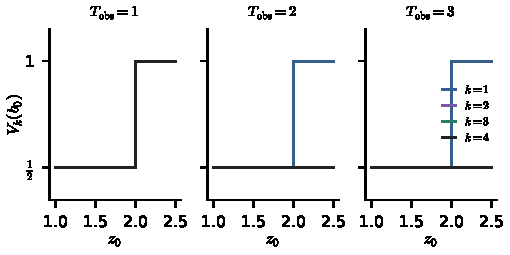
\includegraphics[width=\linewidth]{figs_bs2/fig_staircase.pdf}
\caption{The closed-form values of Proposition \ref{cor:closed} on the
delayed grid: flat at \(\tfrac{1}{2}\) while a branch falls, jumping by
exactly \(\tfrac{1}{2}\) at \(z_{0} = 1 + \min(k, T_{\mathrm{obs}})\),
constant beyond.}
\label{fig:staircase}
\end{figure}

\subsection{The deterministic limit and the two operators}\label{deterministic}

\begin{remark}[the two operators]\label{rem:operators}
The expectation over the disturbance law and the adversarial reading of
its support are \emph{different Bellman operators}. Proposition
\ref{prop:degen} states the deterministic degeneration as a change of
operator: when the kernels are deterministic the stochastic expectation
is replaced by the robust (adversarial-support) reading, and the
resulting value is the robust value of the companion papers. The
degeneration is a theorem about the robust operator; it is not a claim
about the stochastic plant, whose expectation and robust readings differ
in general (Section \ref{scope}).
\end{remark}

\begin{proposition}[survived-mass formula]\label{prop:degen}
Let the kernels be deterministic, \(x^{+} = F(x, a, d)\), and let the
disturbance be read adversarially within its support --- the robust
operator of Remark \ref{rem:operators}. Let the window be blind with
declared sequential class \(\Pi_{B}\). Then the degenerated value is the
\emph{survived-mass formula}
\[
V_{k}(b) = \max_{(u_{0},\dots) \in \Pi_{B}}\;
\sum_{x \in \mathrm{supp}\, b} b(x)\,
\mathbf{1}\bigl[ x \text{ survives } (u_{0}, \dots) \bigr],
\]
a maximum of rational linear functions of \(b\) (the surviving indicators
are the degenerate alpha-vectors). Consequently: if the support \(B\)
carries a jointly surviving blind sequence, \(V_{k}(b) = 1\); and if every
declared sequence loses some branch, then
\(V_{k}(b) \le 1 - \min_{x \in B} b(x)\) --- the robust common-action
verdicts and the minimal-mass deficit bound of the companion papers,
recovered as exact values of the robust operator.
\end{proposition}

With deterministic kernels the posterior support follows the set-valued
recursion, survival from a branch under a fixed sequence is a
deterministic event, and prior mass sums over surviving branches;
maximizing over declared sequences gives the formula, from which both
consequences are immediate (a lost branch carries at least the minimal
mass).

\begin{proposition}[stabilization on the survivable-set lattice]\label{prop:freeze}
With deterministic kernels the survivable-set families satisfy
\(\mathcal{S}_{\ell+1} \subseteq \mathcal{S}_{\ell}\); hence
\(V_{\ell}(b)\) is non-increasing in the horizon and stabilizes after
at most \(2^{|\mathrm{supp}\, b|}\) strict decreases, the frozen value
being \(\max_{S}\, b(S)\) over the maximal sets of the frozen family
--- an exact computable infinite-horizon value. On the delayed instance
the open-loop family is frozen from \(\ell = 1\) (oscillation and
single-branch rises are length-independent), and the declared class
freezes once \(k \ge T_{\mathrm{obs}}\) (the window ends and the
rising continuation \(u = +1\) then preserves safety indefinitely
above the floor); consequently every audited table at
\(T_{\mathrm{obs}} \le 3\), \(k \le 4\) already records the
full-horizon value.
\end{proposition}

Survivability over a longer window is the conjunction of survivability
over the shorter, giving the decreasing lattice; a monotone sequence on a
finite lattice freezes; the instance's length-independence and the
window's end give the two freezing statements, verified to horizon
\(40\) by the verification script.

On the two-floor chance instance --- states \(\{0, 1\}\), actions
\(u \in \{\tfrac{2}{5}, \tfrac{3}{5}\}\), state \(0\) surviving exactly
the lower action and state \(1\) exactly the higher --- the one-step
witness set is \(\Gamma^{\Pi}_{1} = \{(1,0), (0,1)\}\) and
\(V_{k}(b_{0}) = \tfrac{1}{2}\) for all audited \(k \le 5\): the chance
deficit \(\delta = \tfrac{1}{2}\) is attained, and the deficit equals the
minimal mass (Figure \ref{fig:twofloor}).

The asymmetric audit prices the deficit beyond the symmetric case. At
\((z_{0}, T_{\mathrm{obs}}) = (\tfrac{3}{2}, 2)\) with prior masses
\(w = \tfrac{3}{10}\) and \(\tfrac{7}{10}\), the four blind two-step
sequences survive
\(\{ \tfrac{3}{10}, \tfrac{3}{10}, \tfrac{7}{10}, \tfrac{7}{10} \}\)
(Table \ref{tab:masses}): every sequence loses a branch, so
\(V_{2}(b_{0}) = \tfrac{7}{10}\) and the deficit \(\tfrac{3}{10}\) equals
the minimal mass --- the degenerate bound of Proposition
\ref{prop:deficit} attained off the symmetric prior (Figure
\ref{fig:masses}).

\begin{table}[t]
\centering
\footnotesize
\caption{The asymmetric audit at
\((z_{0}, T_{\mathrm{obs}}) = (\tfrac{3}{2}, 2)\),
\(b_{0} = (\tfrac{3}{10}, \tfrac{7}{10})\): survived mass of each blind
two-step sequence. Every sequence loses a branch at step \(1\) --- at
\(z_{0} = \tfrac{3}{2}\) the first move sends one branch to
\(\tfrac{1}{2} < 1\) ---; the value is
\(\tfrac{7}{10}\) and the deficit \(\tfrac{3}{10}\) equals the minimal
mass.}
\label{tab:masses}
\begin{tabular}{@{}l c l@{}}
\toprule
Sequence & Survived mass & Lost branch\\
\midrule
\((+1, +1)\) & $\tfrac{3}{10}$ & heavier branch, step 1\\
\((+1, -1)\) & $\tfrac{3}{10}$ & heavier branch, step 1\\
\((-1, +1)\) & $\tfrac{7}{10}$ & lighter branch, step 1\\
\((-1, -1)\) & $\tfrac{7}{10}$ & lighter branch, step 1\\
\bottomrule
\end{tabular}
\end{table}

\begin{figure}[t]
\centering
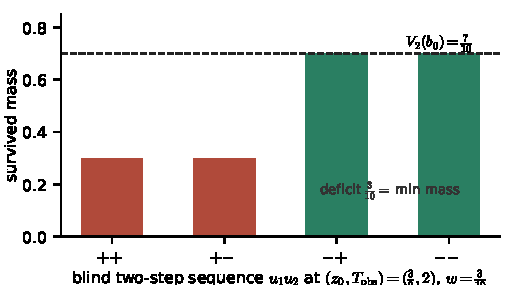
\includegraphics[width=\linewidth]{figs_bs2/fig_masses.pdf}
\caption{The asymmetric audit: survived mass by blind two-step sequence
at \((\tfrac{3}{2}, 2)\) with \(w = \tfrac{3}{10}\). The best sequences
save the heavy branch only; the deficit \(\tfrac{3}{10}\) is the minimal
mass, attained.}
\label{fig:masses}
\end{figure}

\subsection{Certificates as deficit bounds}\label{deficit}

The obstruction certificates bound the deficit from below; their attaining
witnesses are the deficit's dual objects --- computed lower-bound sides of
the exact value, not surrogates for it.

\begin{proposition}[deficit lower bounds]\label{prop:deficit}
Write \(\Delta_{k}(b) = 1 - V_{k}(b)\) for the deficit, and let
\(\mathcal{W}^{\mathrm{bel}}_{k}\)
denote the \(k\)-step robust kernel in belief space: the family of beliefs
whose support admits a jointly surviving declared-class sequence. Each
companion certificate is a computable lower bound on the deficit.
(i) \emph{Chance-constrained common action:} if the one-step violation
probabilities satisfy \(\sum_{x} b(x)\, p(x, a) \ge \delta\) for every
\(a \in A\), then \(\Delta_{k}(b) \ge \delta\) for every \(k \ge 1\).
(ii) \emph{Degenerate minimal mass:} at the deterministic limit, if
\(b \notin \mathcal{W}^{\mathrm{bel}}_{k}\) (the support admits no jointly surviving declared
sequence), then \(\Delta_{k}(b) \ge \min_{x \in \mathrm{supp}\, b} b(x)\)
--- the two-floor instance attains \(\delta = \tfrac{1}{2}\), and on the
delayed grid at \((z_{0}, T_{\mathrm{obs}}) = (\tfrac{3}{2}, 2)\) every
blind sequence loses a branch, so the deficit is at least the minimal
mass \(\tfrac{3}{10}\) of the audited asymmetric prior, attained
(Table \ref{tab:masses}).
(iii) \emph{Monotone deficit:} \(V_{k+1}(b) \le V_{k}(b)\), so the
deficit is non-decreasing in the horizon; on the certified nonviability
region of the delayed grid the declared-class deficit is constant in
\(k\) once \(k > T_{\mathrm{obs}}\) (and at every \(k \ge 1\) on
the common-action cells), while on the timing cells it steps from
\(0\) at \(k = 1\) to \(\tfrac{1}{2}\) at \(k \ge 2\) (Theorem
\ref{thm:agree}d).
For finite horizons the exact deficit
\(1 - \max_{\alpha \in \Gamma_{k}} \alpha^{\top} b\) is computable, and
the bounds are witnesses of it, not surrogates.
\end{proposition}

\subsection{Agreement on the delayed-regime class}\label{agreement}

The delayed hidden-regime instance of the calculus paper --- regimes
\(\theta \in \{-1, +1\}\), blind window \(T_{\mathrm{obs}}\), declared
hold class \(\{u \equiv \pm 1\}\), prior \((\tfrac12, \tfrac12)\) from
\(z_{0}\) --- is the agreement test bed. The class declaration is part of
the model: the blind-window policy may be required to hold one action
throughout the window (the declared hold class), or may act sequentially
without observation, or may act with open-loop time-variation.

\begin{theorem}[certificate--value agreement]\label{thm:agree}
On the audited grid (\(z_{0} \in \{1.0, \dots, 2.5\}\),
\(T_{\mathrm{obs}} \in \{1,2,3\}\); 48 cells), over the declared hold
class, and horizons \(k \le 4\):
(a) the segment-form enumeration of the declared hold class
(Proposition \ref{prop:pl}, segment form) returns exactly the closed
form of Proposition
\ref{cor:closed} (on the audited grid the second indicator of the
\(k \le T_{\mathrm{obs}}\) line is vacuous, \(z_{0} + k \ge 2\); it is
retained for branch symmetry). The class constraint is load-bearing
here: a stagewise recursion over \(A(\Pi) = \{\pm 1\}\) would compute
the unrestricted value, which is \(1\) on the timing cells --- the
agreement is a statement about the segment enumeration;
(b) the certificate partition coincides with the value boundaries:
``viable'' iff \(V_{k} \equiv 1\); common-action-certified iff
\(V_{1}(b_{0}) < 1\); timing-certified iff \(V_{1}(b_{0}) = 1\) but
\(V_{T_{\mathrm{obs}}+1}(b_{0}) < 1\);
(c) at the one-step horizon both mirror witnesses \((1,0)\) and
\((0,1)\) attain the value \(\tfrac{1}{2}\) below \(z_{0} = 2\), and
the merged \((1,1)\) attains \(1\) at and above it; at horizon
\(k \le T_{\mathrm{obs}}\) the family changes at \(z_{0} = 1 + k\) ---
an off-grid consequence of the closed form (in particular \(z_{0} = 3\),
not \(2\), for \(k = 2\) with \(T_{\mathrm{obs}} \ge 2\)), verified
by the verification script beyond the audited grid, which stops at
\(z_{0} = 2.5\); and read as a function of
the continuous parameter \(z_{0}\) the hold-class value has jump
discontinuities exactly at \(z_{0} = 1 + \min(k, T_{\mathrm{obs}})\) --- a
jump of exactly \(\tfrac{1}{2}\), from \(\tfrac{1}{2}\) to \(1\) --- these
loci being the certificate edges on the grid (kinks in the strict sense
belong to the piecewise-linear value as a function of the belief, not of
\(z_{0}\));
(d) on the nonviable cells the hold-class deficit equals
\(\tfrac{1}{2}\) at every horizon \(k > T_{\mathrm{obs}}\) and at
every \(k \le T_{\mathrm{obs}}\) with \(k > z_{0} - 1\), while it is
\(0\) at horizons \(k \le z_{0} - 1\) (on the audited grid: on the
timing cells the deficit is \(0\) at \(k = 1\) and \(\tfrac{1}{2}\)
at \(k \ge 2\); on the common-action cells it is \(\tfrac{1}{2}\) at
every \(k \ge 1\)) --- the minimal-mass bound attained with the
minimal prior from the first horizon at which the falling branch
exits.
\end{theorem}

\begin{proof}[Derivation of the jump loci]
Fix \(T_{\mathrm{obs}}\) and \(k\). On the closed form: if
\(k \le T_{\mathrm{obs}}\) the value is
\(\tfrac{1}{2}(\mathbb{1}[z_{0} \ge 1 + k] + 1)\), the second indicator
being identically one on the grid; it jumps by exactly \(\tfrac{1}{2}\)
at \(z_{0} = 1 + k\). If \(k > T_{\mathrm{obs}}\) the value is
\(\tfrac{1}{2}(1 + \mathbb{1}[z_{0} \ge 1 + T_{\mathrm{obs}}])\),
jumping by exactly \(\tfrac{1}{2}\) at \(z_{0} = 1 + T_{\mathrm{obs}}\).
Both loci are \(z_{0} = 1 + \min(k, T_{\mathrm{obs}})\); between jumps
both expressions are constant in \(z_{0}\). The witness family changes
exactly at the same loci: the attaining one-step vectors are both
mirrors \((1, 0)\) and \((0, 1)\) below \(z_{0} = 2\) and the merged
\((1, 1)\) at and above, and at horizon \(k\) the change
sits at \(z_{0} = 1 + \min(k, T_{\mathrm{obs}})\).
\end{proof}

\begin{theorem}[class lattice and realized gaps]\label{thm:lattice}
For the value of Definition \ref{def:value}, \(\Pi \subseteq \Pi'\)
implies \(V^{\Pi}_{k}(b) \le V^{\Pi'}_{k}(b)\). On the delayed
instance with \(\ell \ge 1\) and \(z_{0} \ge 1\):
\[
V^{\Pi_{\mathrm{hold}}} \;\le\; V^{\Pi_{\mathrm{ol}}}
\;=\; V^{\Pi_{\mathrm{seq, blind}}}
\;\le\; V^{\Pi_{\mathrm{obs}}},
\]
the middle equality holding because no observation arrives inside the
window, so sequential blind policies reduce to open-loop sequences; and
\(V^{\Pi_{\mathrm{obs}}} = \mathbb{1}[z_{0} \ge 1]\) (the controller
knows \(\theta\) at \(t = 0\) and plays the rising control). The gaps
are exact: \(V^{\Pi_{\mathrm{ol}}} - V^{\Pi_{\mathrm{hold}}} =
1 - \max(w, 1 - w)\) exactly on \(\{2 \le z_{0} < 1 + \ell\}\) ---
the \emph{value of flexibility} --- and
\(V^{\Pi_{\mathrm{obs}}} - V^{\Pi_{\mathrm{ol}}} = 1 - \max(w, 1 -
w)\) exactly on \(\{1 \le z_{0} < 2\}\) --- the \emph{value of
observation}; at the symmetric prior each gap is \(\tfrac12\) on its
cells and \(0\) elsewhere, and the two cell families are disjoint.
\end{theorem}

Inclusion monotonicity is immediate from the maximizing definition; the
instance values are Theorem \ref{thm:parametric}'s and the observed
value is the rising computation; the gap arithmetic is
\(1 - \max(w, 1 - w) = \min(w, 1 - w)\).

\begin{theorem}[class declaration]\label{thm:class}
The declared hold class and the unrestricted sequential blind class
coincide at the one-step horizon. For horizons \(k \ge 2\) they differ
exactly where \(2 \le z_{0} < 1 + \min(k, T_{\mathrm{obs}})\) --- on
the audited grid \((z_{0} \le 2.5)\) exactly the timing cells, since
\(1 + \min(k, T_{\mathrm{obs}}) \ge 3\) there --- and there open-loop
time-variation within the blind window lifts the value to one: an
alternating hold sequence keeps both branches at or above the floor
whenever \(z_{0} \ge 2\), which no constant hold does (off the grid
the hold class already attains one at \(z_{0} \ge 1 + k\): e.g. at
\((z_{0}, T_{\mathrm{obs}}, k) = (3.5, 3, 2)\) both classes attain
one, so no difference). On the
common-action cells \(z_{0} < 2\) the restriction costs nothing --- no
blind sequence saves both branches --- and on the viable cells both
classes attain one. On the audited grid the difference comprises exactly
the 12 timing cells at each of \(k = 2, 3, 4\): 36 cell-horizon
combinations in all (Figure \ref{fig:classdiff}).
\end{theorem}

\begin{proof}[Derivation of Theorem \ref{thm:class}]
At \(k = 1\) both classes choose one blind action, so they coincide. Let
\(k \ge 2\) and write the two branch positions after a blind sequence
\(u_{1:\ell}\), \(\ell = \min(k, T_{\mathrm{obs}})\), as
\(z_{0} \pm \sum_{t} u_{t}\). If \(z_{0} < 2\), some branch sits below
\(2 - (z_{0} - 1)\) steps from its floor, and since the partial sums of
any \(\pm1\)-sequence move one branch down whenever they move the other
up, one branch reaches its floor: no blind sequence saves both, both
classes give \(\tfrac{1}{2}\), no difference. If
\(z_{0} \ge 1 + \min(k, T_{\mathrm{obs}})\) the constant hold already
survives the window on both branches (the falling branch exits only
after \(k > z_{0} - 1\) steps) and both classes attain one. On the
difference cells \(2 \le z_{0} < 1 + \min(k, T_{\mathrm{obs}})\): a
constant hold drives the
falling branch to \(z_{0} - \ell < 1\) (deficit), while the alternating
sequence has partial sums in \(\{0, \pm 1\}\), so both branches stay at
or above \(z_{0} - 1 \ge 1\) through the window, and revelation at
\(T_{\mathrm{obs}}\) then regenerates both: the unrestricted class
attains one while the declared class does not. This locates the
difference setwise.
\end{proof}

\begin{remark}[the timing obstruction is class-scoped]\label{rem:scope}
The calculus paper's timing certificates --- \(\sigma^{*}(B_{0}) =
z_{0} - 1\), with the certificate firing exactly when
\(T_{\mathrm{obs}} > \sigma^{*}\) (equivalently
\(z_{0} < 1 + T_{\mathrm{obs}}\); viability at the deadline holds when
\(T_{\mathrm{obs}} \le \sigma^{*}\)) --- are statements about the
declared hold-until-review class --- the institutional reading of a
sampled-review regulator. Theorem \ref{thm:class} quantifies the
contrast: within the declared class the timing cells are nonviable with
deficit \(\tfrac{1}{2}\) at every horizon \(k \ge 2\) (and \(0\) at
\(k = 1\)); under the unrestricted sequential blind class the same
cells attain value \(1\) by oscillation, and on the audited grid no
other cell differs. The
timing obstruction therefore certifies exactly what it claims ---
nonviability \emph{within the declared class} --- and no statement of the
companion papers is altered by this reading. The word ``adaptive'' is
avoided for blind windows: while the window is blind, no observation
updates the belief, and the only distinction available is hold-constant
versus time-varying open-loop control.
\end{remark}

\begin{figure}[t]
\centering
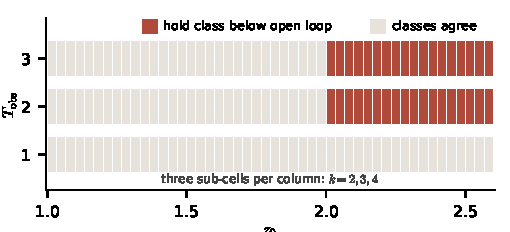
\includegraphics[width=\linewidth]{figs_bs2/fig_classdiff.pdf}
\caption{The class declaration on the audited grid: red cells mark
cell-horizon combinations where the declared hold class and the
unrestricted open-loop class differ --- exactly the timing cells
(\(2 \le z_{0} < 1 + T_{\mathrm{obs}}\)) at horizons \(k = 2, 3, 4\)
(three sub-cells per column); 36 combinations in all. The classes agree
at \(k = 1\), on the common-action cells, and on the viable cells.}
\label{fig:classdiff}
\end{figure}

\subsection{Adaptive observation and hidden parameters}\label{adaptive}

Observation is a design variable. Structural uncertainty --- a hidden
parameter resolved too late, rather than noisy data --- is the
obstruction: the state augments with a hidden parameter
\(\theta \in \Theta\), the belief lives on the product
\((x, \theta)\), and the obstruction is the emptiness of the joint
floor-servable set over \((x, \theta)\) cells. On the declining instance
the parameter \(\theta \in \{-1, +1\}\) gates the correctable component
of a \(-\tfrac{1}{10}\) drift; the list of affected sustainability
parameters --- regeneration rates, climate sensitivity, institutional
effectiveness --- motivates the model class, and the paper verifies on
exact instances.

\begin{proposition}[probes and learning deadlines]\label{prop:learn}
On the audited grid, with quantized control \(u \in \{-1, 0, 1\}\) and
hold-then-probe-then-act schedules: with \(\theta\) observed, every cell
is viable (16 of 16). Under one-probe endogenous learning with free probe timing (probe at
the start), the probe
reveals \(\theta\) exactly --- the branch separation is \(2\), so one
observation splits the belief with no statistics --- and survival forces
\(z_{0} \ge 21/10\), independent of any deadline. Under the audited
pinned-probe family --- hold \(u = 0\) to the probe horizon and probe
at \(T_{\mathrm{learn}}\), so no earlier probe is available within the
family --- viability holds exactly when
\[
z_{0} \;\ge\; \frac{21}{10} \;+\; \frac{T_{\mathrm{learn}}}{10},
\qquad T_{\mathrm{learn}} = 0, 1, 2, 3, 4,
\]
the pinned-probe learning-deadline identity: the deadline prices the
forced late probe, and the kernel shrinks exactly
linearly and antitone in it, \(|K| = 5, 4, 3, 2, 1\) on the grid for
\(T_{\mathrm{learn}} = 0, 1, 2, 3, 4\) (Table \ref{tab:deadline} and
Figure \ref{fig:deadline}). Two exact benchmarks bound the family from
both sides: with free probe timing the threshold is flat at
\(21/10\), and with probe-free exogenous revelation at
\(T_{\mathrm{learn}}\) (hold, then the learned act; no probe)
viability holds exactly when \(z_{0} \ge 1 + T_{\mathrm{learn}}/10\)
--- kernel sizes \(16, 15, 14, 13, 12\) on the grid for
\(T_{\mathrm{learn}} = 0, 1, 2, 3, 4\); the audited family sits
between the two. A two-patch instance with unknown
regeneration rate \(g \in \{1, 2\}\) shows the same phenomenon on the
audited two-patch belief pair: unknown-regeneration nonviable,
\((x, g)\)-observed viable.
\end{proposition}

\begin{proof}
The schedule pins the probe to \(T_{\mathrm{learn}}\): within the
family no earlier probe is admissible, so the free-probe and probe-free
thresholds are not attainable in it. Before \(T_{\mathrm{learn}}\) the
drift is \(-\tfrac{1}{10}\) (hold
\(u=0\)), so survival to the probe forces
\(z_{0}-\tfrac{T_{\mathrm{learn}}}{10}\ge\) the probe threshold; the
probe \(u=+1\) moves \(z\) by \(-\tfrac{1}{10}+\theta\), which must stay
safe on both branches, giving the threshold \(\tfrac{21}{10}\) at
\(T_{\mathrm{learn}}=0\); after the probe the learned law \(u=\theta\)
has drift \(-\tfrac{1}{10}+\theta^2=\tfrac{9}{10}>0\), so survival is
indefinite. The branch positions
\(z_{0}-\tfrac{1}{10}T_{\mathrm{learn}}-\tfrac{1}{10}\pm1\) differ by
\(2\), so the post-probe reading determines \(\theta\) uniquely.
Antitonicity is the threshold identity; strictness on the grid is the
computed counts \(5,4,3,2,1\).
\end{proof}

\begin{table}[t]
\centering
\footnotesize
\caption{The pinned-probe learning-deadline audit: the exact threshold
\(\tfrac{21}{10} + \tfrac{T_{\mathrm{learn}}}{10}\) and the resulting
kernel on the grid at each deadline.}
\label{tab:deadline}
\begin{tabular}{@{}l c c l@{}}
\toprule
\(T_{\mathrm{learn}}\) & Threshold & \(|K|\) & Kernel \(K\) on the grid\\
\midrule
0 & $21/10$ & 5 & $\{2.1, 2.2, 2.3, 2.4, 2.5\}$\\
1 & $22/10$ & 4 & $\{2.2, 2.3, 2.4, 2.5\}$\\
2 & $23/10$ & 3 & $\{2.3, 2.4, 2.5\}$\\
3 & $24/10$ & 2 & $\{2.4, 2.5\}$\\
4 & $25/10$ & 1 & $\{2.5\}$\\
\bottomrule
\end{tabular}
\end{table}

\begin{figure}[t]
\centering
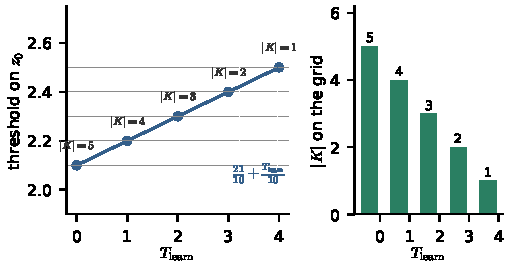
\includegraphics[width=\linewidth]{figs_bs2/fig_deadline.pdf}
\caption{The pinned-probe learning-deadline identity: the viability
threshold increases exactly linearly in \(T_{\mathrm{learn}}\) (left),
and the kernel on the grid shrinks linearly and antitone, \(|K| = 5, 4,
3, 2, 1\) (right); the probe-free benchmark \(1 +
T_{\mathrm{learn}}/10\) (kernels \(16\) down to \(12\)) and the
flat free-probe threshold \(21/10\) bound it from below and above.}
\label{fig:deadline}
\end{figure}

\begin{figure}[t]
\centering
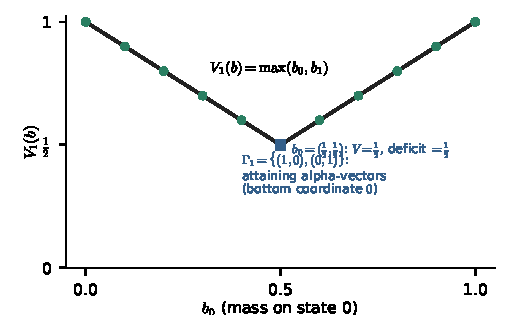
\includegraphics[width=0.88\linewidth]{figs_bs2/fig_twofloor.pdf}
\caption{The two-floor chance instance: the one-step value is
\(\max(b_{0}, b_{1})\), attained by the alpha-vectors of
\(\Gamma^{\Pi}_{1} = \{(1,0), (0,1)\}\) with zero bottom coordinate (green
probes); at the symmetric prior the value is \(\tfrac{1}{2}\) and the
deficit equals the minimal mass.}
\label{fig:twofloor}
\end{figure}

\subsection{Genuinely stochastic instances}\label{stochastic}

Everything to this point has deterministic kernels and observations; the
values are prior masses of surviving branches. This section opens the
stochastic layer, where values cease to be two-valued and the min-mass
bound ceases to be universal.

\begin{proposition}[weighted-path deficit identity]\label{prop:pathdeficit}
At the one-step horizon, with finite \(X\), deterministic per-reading
actions \(a(y')\), and arbitrary normalized observations, the deficit
is exactly
\[
\Delta_{1}(b) \;=\; \sum_{x} b(x)\, p_{x},
\qquad p_{x} = \mathbb{P}\bigl(a(y') \text{ unsafe at } x \,\big|\, x\bigr),
\]
the prior mass weighted by fatal-reading probabilities. The min-mass
bound is the case \(p_{x} \equiv 1\) (deterministic readings, no
common action) and is \emph{not universal}: in the two-state instance
with \(a_{i}\) safe only at \(x_{i}\) and sensor error \(\varepsilon\)
(\(\mathbb{P}(\text{reads } j \ne i \mid x_{i}) = \varepsilon\)),
the deficit is \(\varepsilon\) for every prior; at
\(b = (\tfrac12, \tfrac12)\), \(\varepsilon = \tfrac1{20}\), the
deficit \(\tfrac1{20}\) is strictly below the minimal mass
\(\tfrac12\).
\end{proposition}

\begin{proposition}[noisy probes and the repetition trade-off]\label{prop:noisyprobe}
On the declining instance (blind drift \(-\tfrac1{10}\)), pin a single
probe to horizon \(t_{p}\) whose reading is correct with probability
\(1 - \varepsilon\) and flipped with probability \(\varepsilon\),
then act on the reading to horizon \(k \ge t_{p}\). With
\(z_{p} = z_{0} - t_{p}/10\):
\[
V_{k}(b_{0}) \;=\; (1 - \varepsilon)\,\mathbb{1}[z_{p} \ge 1]
\;+\; \varepsilon\,\mathbb{1}\bigl[z_{p} \ge 1 + \tfrac{11}{10}(k - t_{p})\bigr],
\]
exactly (the correct reading acts under drift \(\tfrac9{10}\), the
flipped reading under drift \(-\tfrac{11}{10}\)). The values realize
exactly three levels \(\{0,\, 1 - \varepsilon,\, 1\}\) ---
genuinely non-two-valued --- and the min-mass bound survives here as a
bound (the deficit \(\varepsilon\) or \(1\) dominates the
post-probe minimal mass \(\varepsilon\)) while failing as an
identity. With three pinned probes and majority reading, the
wrong-majority probability is
\(3\varepsilon^{2}(1 - \varepsilon) + \varepsilon^{3} = \varepsilon^{2}(3 - 2\varepsilon)\)
--- \(\tfrac{7}{250}\) at \(\varepsilon = \tfrac1{10}\), against
\(\tfrac1{10}\) for one probe --- and the same display holds with
\(p = \tfrac{7}{250}\) in place of \(\varepsilon\): each
additional probe step costs \(\tfrac1{10}\) of floor margin to the
blind drift, the exact explore--exploit exchange at this scale.
\end{proposition}

\begin{proof}
Condition on \((\theta, \text{reading})\): the four joint cases carry
probabilities \(\tfrac12(1-\varepsilon)\) and \(\tfrac12\varepsilon\)
per branch; the correct reading acts under drift
\(-\tfrac1{10} + \theta^{2} = \tfrac9{10}\) and survives from
\(z_{p} \ge 1\); the flipped reading acts under drift
\(-\tfrac1{10} - 1 = -\tfrac{11}{10}\) and survives exactly when
\(z_{p} - \tfrac{11}{10}(k - t_{p}) \ge 1\); summing gives the
display. For the majority family, the wrong-majority event is two or
three flipped readings, of probability
\(3\varepsilon^{2}(1-\varepsilon) + \varepsilon^{3}\); the falling
continuation is as above. The identity's proof is the law of total
probability over readings at the one-step horizon.
\end{proof}

\subsection{Verification methods}\label{methods}

Every value, bound, identity, threshold, figure, and tabulated entry in
this paper is regenerated by deterministic scripts in exact integer and
rational arithmetic, standard library only. Three per-system scripts
cover the audited instances, and one master entry point chains them.
The belief-state campaign script runs sixteen check families on the
stochastic values (the two-floor instance, piecewise-linearity, the
deterministic limit, the 48-cell agreement, the partition coincidence,
the witness family, the deficit identity, the unrestricted class,
rationality of all 384 campaign alpha-vectors, deficit monotonicity, the
oscillation identity, model completeness, the selector split, dimension
consistency, the jump loci, and the declarations), chaining two
per-instance scripts of twenty-one further checks. The stochastic
selector script re-derives every selector claim in fifteen check
families (S1--S15: the two-floor backup, eleven-belief piecewise
linearity, degeneration against brute force, 48-cell closed-form
agreement, partition coincidence, witness-family loci, the exact
deficit on all 42 nonviable cells, the class declaration by brute
force, rationality of the 384 vectors, monotonicity, the oscillation
identity to horizon 24, model completeness, the selector split,
dimension padding, and the one-sided jump values). The hidden-parameter
script runs six check families on the adaptive-observation instance
(theta observed on all 16 cells, the probe threshold
\(\tfrac{21}{10}\) as a branchwise identity, the deadline identity at
\(T_{\mathrm{learn}} = 0, \dots, 4\), injective revelation, the
antitone kernel chain, and the unknown-regeneration two-patch
instance). The master script for this paper chains the three, then
recomputes independently from the definitions: the closed-form values on
the whole \(16 \times 12\) grid by direct branch-mass enumeration, the
resulting census (\(36\) unit values and \(156\) half values on the
declared class), the identity of the class-difference set with the region
\(2 \le z_{0} < 1 + \min(k, T_{\mathrm{obs}})\), checked on an
extended grid to \(z_{0} = 4.0\) and equal to the timing-cell
combinations on the audited grid at \(k \ge 2\), by brute-force
enumeration over blind sequences; the \(384\)-vector type census
(\(156\), \(156\), \(72\)) and its deduplicated \(348\)-vector
form; the hold-class deficit profile on all 48 cells (\(0\) before the
falling-branch exit, \(\tfrac{1}{2}\) after); the lost-branch step of
the asymmetric audit (step \(1\) for all four sequences, heavier
branch under \(u_{1} = +1\), lighter under \(u_{1} = -1\)); the
pinned-probe learning-deadline chain
\(\tfrac{21}{10} + \tfrac{T_{\mathrm{learn}}}{10}\) with the
free-probe (\(21/10\), flat) and probe-free
(\(1 + T_{\mathrm{learn}}/10\), kernels \(16\) down to \(12\))
benchmarks; and every headline
number asserted present in the text and bound to the chained scripts'
certified families. Two independent paths back the closed forms: a
brute-force path that enumerates trajectories straight from the
definitions (all holds and all open-loop sequences, pathwise survival)
over a structured sweep of 2268 triples
\((z_{0}, w, \ell)\) including \(z_{0} < 1\), and a seeded
randomized battery of 500 further cases; the survivable-set antichain,
the class ordering and its gaps, the stabilization freeze (spot
enumeration to horizon \(15\) and value agreement to horizon
\(40\)), the weighted-path identity, the sensor counterexample, and
the noisy-probe and majority closed forms are each re-derived by
independent enumeration.

\subsection{Delimitations and outlook}\label{scope}

The semantics here is stochastic expectation: the value is a survival
\emph{probability}, and the robust quantifiers of the companion papers
are recovered only at the deterministic degeneration, which is a change
of operator (Remark \ref{rem:operators}); the stochastic and robust
readings of a genuinely stochastic plant differ, and this paper does not
conflate them. The timing layer's statements, here and in the companion
papers, are class-scoped (Remark \ref{rem:scope}). No learning theory is
claimed beyond the one-probe exact split: Bayesian updating, repeated
experiments, and exploration--exploitation trade-offs are out of scope;
the deadline identity is for the pinned-probe schedule family (hold to
the probe horizon, probe, learned act), with the free-probe and
probe-free benchmarks stated alongside, and other schedules are not
classified; the parameter
\(\theta\) enters additively, and state-dependent parameter dynamics
belong to the hybrid companion's setting. The alpha-set growth is
exponential in the worst case --- and finite-horizon partially
observable problems are PSPACE-complete, their no-observation variant
NP-complete (Papadimitriou and Tsitsiklis, 1987) --- so the audited
two-witness families are structural, not representative. The
distributionally robust interpolation between the expected and
adversarial operators over moment- or distance-based ambiguity sets
(piecewise-linear values persist there; Nakao, Jiang, and Shen, 2021) is
the formal home of any worst-case wording and is not developed here.
Scaling past the audited instances --- exact point-based value iteration
with rational solvers, survivable-set compression over the antichain of
Proposition \ref{prop:antichain}, and medium instances with several
hidden parameters --- the probe-count asymptotics of the repetition
trade-off, the general learning-deadline law for additively entering
hidden parameters, and a proof-assistant formalization of the closed
forms are the natural next steps; the deficit-bound reading of
Proposition \ref{prop:deficit} remains the interface through which this
theory attaches to the certificate families already established, and the
exact rational values of the audited campaign are the benchmark any
relaxation must meet.

\subsection{Conclusion}\label{conclusion}

The belief-state safety value carries the obstruction calculus into the
probabilistic setting without loss of exactness. The support identity
ties the value-one level to the viable-set recursion; rational
alpha-vectors keep every audited value exact, and the complete value
table shows the two-valued structure the certificates predict; the
certificates survive as deficit lower bounds, attained on natural
instances on both the symmetric and the asymmetric prior; the audited
delayed-regime class agrees with its closed form cell by cell, with the class declaration responsible for exactly the 36 timing
combinations on the grid; and the adaptive-observation audit prices late resolution exactly ---
for the pinned-probe family a linear learning deadline on the viable
set, \(|K| = 5, 4, 3, 2, 1\), bracketed by the flat free-probe
threshold and the probe-free benchmark --- while the stochastic layer
prices observation noise exactly: a weighted-path deficit identity, a
sensor instance breaking the min-mass bound's universality, and a
repetition trade-off at \(7/250\) per extra probe pair. The
observation layer, not the forecast layer, sets the value; the design
rules are the same ones the deterministic audits impose, now with a
price attached and every number in the tables open to script-level
re-inspection.

\subsection*{References}

{\footnotesize
Abaee, A. An obstruction calculus for viability under incomplete
observation (submitted).

Abaee, A., 2026a. Robust viability of the 2J3KL limit reference point
under a surplus-production map: policy scoring, expansion, and when
catch cannot help. Zenodo.
\url{https://doi.org/10.5281/zenodo.22552060}

Bertsekas, D.P., Shreve, S.E., 1978. Stochastic Optimal Control: The
Discrete-Time Case. Academic Press, New York.

\`{A}str\"{o}m, K.J., 1965. Optimal control of Markov processes with
incomplete state information. J. Math. Anal. Appl. \textbf{10},
174--205.

Alshiekh, M., Bloem, R., Ehlers, R., K\"{o}nighofer, B., Niekum, S.,
Topcu, U., 2018. Safe reinforcement learning via shielding. Proc. AAAI
Conf. Artif. Intell. \textbf{32}(1).

Chatterjee, K., Doyen, L., Henzinger, T.A., 2009. Qualitative analysis
of partially-observable Markov decision processes. In: Int. Symp. Math.
Found. Comput. Sci. (MFCS 2009). LNCS, vol. 5734, pp. 635--646.

Nakao, H., Jiang, R., Shen, S., 2021. Distributionally robust partially
observable Markov decision process with moment-based ambiguity. SIAM J.
Optim. \textbf{31}(1), 461--488.

Papadimitriou, C.H., Tsitsiklis, J.N., 1987. The complexity of Markov
decision processes. Math. Oper. Res. \textbf{12}(3), 441--450.

Smallwood, R.D., Sondik, E.J., 1973. The optimal control of partially
observable Markov processes over a finite horizon. Oper. Res.
\textbf{21}(5), 1071--1088.
}

\subsection*{Declarations}

\subsection*{Funding}
None.

\subsection*{Competing interests}
None.

\subsection*{Data availability}
No external data were used.

\subsection*{Code availability}
The verification script
\url{paper2_probabilistic_sufficiency_v3_verification.py} --- which chains
the per-system scripts \url{paper2_belief_state_v2_verification.py},
\url{paper2_stochastic_selector_v2_verify.py}, and
\url{hidden_parameter_learning_v1_verify.py} --- and the figure-and-table
generation script \url{paper2_belief_state_figures.py} are publicly
available at \url{https://github.com/MIKEAA2020/general-sustainability}
(folder \texttt{arena agent 1/paper rewrites/latex}, at the commit
pinned to this article's submission); they reproduce all values, bounds,
thresholds, figures, and tabulated entries verbatim.

\subsection*{AI declaration}
GLM (Z.ai), Qwen (Alibaba Cloud) and DeepSeek AI assisted with drafting
and iterative review. The author reviewed and edited outputs and takes
responsibility for the final work.

\end{document}
